% Figure: Era Breakdown of the Sutra Corpus
% Data source: Sutra Pipeline database, 17,956 high-relevance papers
% Usage: % Figure: Era Breakdown of the Sutra Corpus
% Data source: Sutra Pipeline database, 17,956 high-relevance papers
% Usage: % Figure: Era Breakdown of the Sutra Corpus
% Data source: Sutra Pipeline database, 17,956 high-relevance papers
% Usage: % Figure: Era Breakdown of the Sutra Corpus
% Data source: Sutra Pipeline database, 17,956 high-relevance papers
% Usage: \input{figures/era-breakdown.tex}

\begin{figure}[t]
\centering
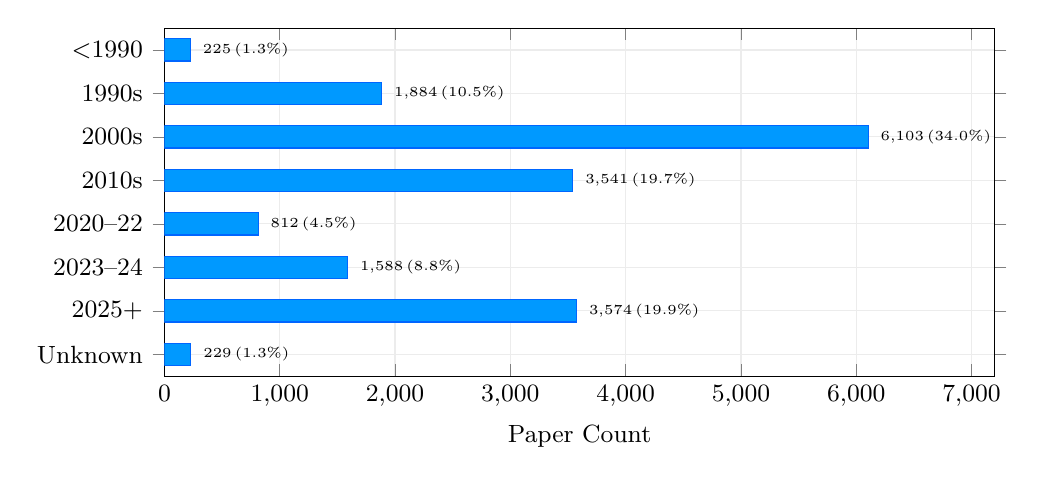
\begin{tikzpicture}
\begin{axis}[
    xbar,
    width=\columnwidth,
    height=6cm,
    xlabel={Paper Count},
    xlabel style={font=\small},
    xmin=0, xmax=7200,
    ytick=data,
    yticklabels={
        {$<$1990},
        {1990s},
        {2000s},
        {2010s},
        {2020--22},
        {2023--24},
        {2025+},
        {Unknown}
    },
    yticklabel style={font=\small},
    y dir=reverse,
    bar width=8pt,
    nodes near coords,
    nodes near coords style={font=\tiny, anchor=west},
    every node near coord/.append style={xshift=1pt},
    enlarge y limits={abs=0.5},
    grid=major,
    grid style={gray!15},
    xticklabel style={font=\small},
    point meta=explicit symbolic,
]
\addplot[fill=blue!40!cyan, draw=blue!60!cyan] coordinates {
    (225,0)  [225\,(1.3\%)]
    (1884,1) [1{,}884\,(10.5\%)]
    (6103,2) [6{,}103\,(34.0\%)]
    (3541,3) [3{,}541\,(19.7\%)]
    (812,4)  [812\,(4.5\%)]
    (1588,5) [1{,}588\,(8.8\%)]
    (3574,6) [3{,}574\,(19.9\%)]
    (229,7)  [229\,(1.3\%)]
};
\end{axis}
\end{tikzpicture}
\caption{\textbf{Era breakdown} of the 17,956 high-relevance papers in the
Sutra Corpus. The 2000s peak (34\%) reflects classical MAS's golden age.
The 2010s dip precedes the LLM-agent explosion (2025+: 19.9\%).
Data source: Sutra Pipeline database.}
\label{fig:era-breakdown}
\end{figure}


\begin{figure}[t]
\centering
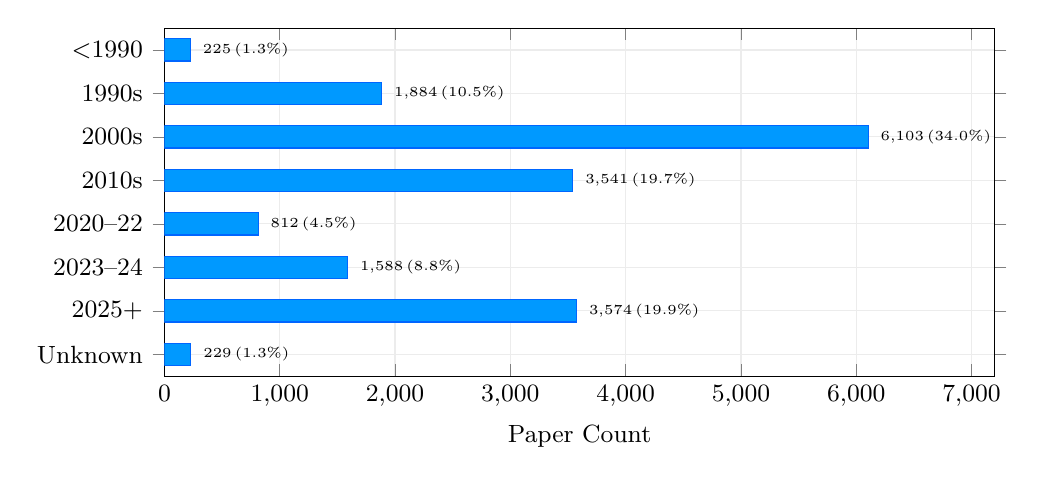
\begin{tikzpicture}
\begin{axis}[
    xbar,
    width=\columnwidth,
    height=6cm,
    xlabel={Paper Count},
    xlabel style={font=\small},
    xmin=0, xmax=7200,
    ytick=data,
    yticklabels={
        {$<$1990},
        {1990s},
        {2000s},
        {2010s},
        {2020--22},
        {2023--24},
        {2025+},
        {Unknown}
    },
    yticklabel style={font=\small},
    y dir=reverse,
    bar width=8pt,
    nodes near coords,
    nodes near coords style={font=\tiny, anchor=west},
    every node near coord/.append style={xshift=1pt},
    enlarge y limits={abs=0.5},
    grid=major,
    grid style={gray!15},
    xticklabel style={font=\small},
    point meta=explicit symbolic,
]
\addplot[fill=blue!40!cyan, draw=blue!60!cyan] coordinates {
    (225,0)  [225\,(1.3\%)]
    (1884,1) [1{,}884\,(10.5\%)]
    (6103,2) [6{,}103\,(34.0\%)]
    (3541,3) [3{,}541\,(19.7\%)]
    (812,4)  [812\,(4.5\%)]
    (1588,5) [1{,}588\,(8.8\%)]
    (3574,6) [3{,}574\,(19.9\%)]
    (229,7)  [229\,(1.3\%)]
};
\end{axis}
\end{tikzpicture}
\caption{\textbf{Era breakdown} of the 17,956 high-relevance papers in the
Sutra Corpus. The 2000s peak (34\%) reflects classical MAS's golden age.
The 2010s dip precedes the LLM-agent explosion (2025+: 19.9\%).
Data source: Sutra Pipeline database.}
\label{fig:era-breakdown}
\end{figure}


\begin{figure}[t]
\centering
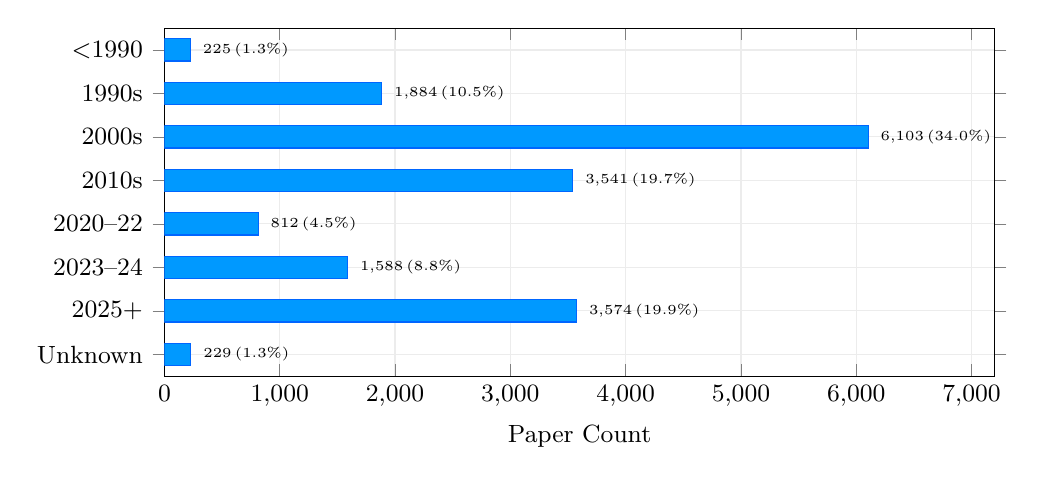
\begin{tikzpicture}
\begin{axis}[
    xbar,
    width=\columnwidth,
    height=6cm,
    xlabel={Paper Count},
    xlabel style={font=\small},
    xmin=0, xmax=7200,
    ytick=data,
    yticklabels={
        {$<$1990},
        {1990s},
        {2000s},
        {2010s},
        {2020--22},
        {2023--24},
        {2025+},
        {Unknown}
    },
    yticklabel style={font=\small},
    y dir=reverse,
    bar width=8pt,
    nodes near coords,
    nodes near coords style={font=\tiny, anchor=west},
    every node near coord/.append style={xshift=1pt},
    enlarge y limits={abs=0.5},
    grid=major,
    grid style={gray!15},
    xticklabel style={font=\small},
    point meta=explicit symbolic,
]
\addplot[fill=blue!40!cyan, draw=blue!60!cyan] coordinates {
    (225,0)  [225\,(1.3\%)]
    (1884,1) [1{,}884\,(10.5\%)]
    (6103,2) [6{,}103\,(34.0\%)]
    (3541,3) [3{,}541\,(19.7\%)]
    (812,4)  [812\,(4.5\%)]
    (1588,5) [1{,}588\,(8.8\%)]
    (3574,6) [3{,}574\,(19.9\%)]
    (229,7)  [229\,(1.3\%)]
};
\end{axis}
\end{tikzpicture}
\caption{\textbf{Era breakdown} of the 17,956 high-relevance papers in the
Sutra Corpus. The 2000s peak (34\%) reflects classical MAS's golden age.
The 2010s dip precedes the LLM-agent explosion (2025+: 19.9\%).
Data source: Sutra Pipeline database.}
\label{fig:era-breakdown}
\end{figure}


\begin{figure}[t]
\centering
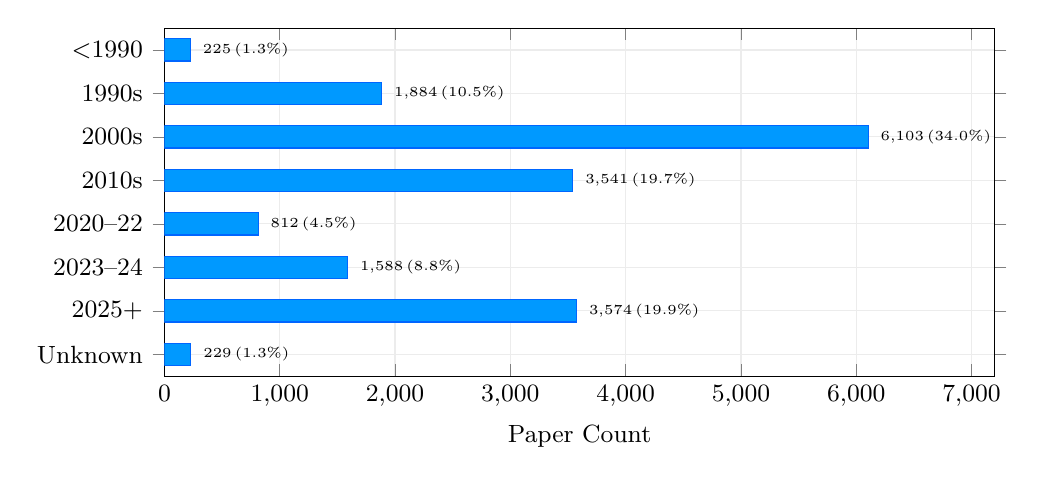
\begin{tikzpicture}
\begin{axis}[
    xbar,
    width=\columnwidth,
    height=6cm,
    xlabel={Paper Count},
    xlabel style={font=\small},
    xmin=0, xmax=7200,
    ytick=data,
    yticklabels={
        {$<$1990},
        {1990s},
        {2000s},
        {2010s},
        {2020--22},
        {2023--24},
        {2025+},
        {Unknown}
    },
    yticklabel style={font=\small},
    y dir=reverse,
    bar width=8pt,
    nodes near coords,
    nodes near coords style={font=\tiny, anchor=west},
    every node near coord/.append style={xshift=1pt},
    enlarge y limits={abs=0.5},
    grid=major,
    grid style={gray!15},
    xticklabel style={font=\small},
    point meta=explicit symbolic,
]
\addplot[fill=blue!40!cyan, draw=blue!60!cyan] coordinates {
    (225,0)  [225\,(1.3\%)]
    (1884,1) [1{,}884\,(10.5\%)]
    (6103,2) [6{,}103\,(34.0\%)]
    (3541,3) [3{,}541\,(19.7\%)]
    (812,4)  [812\,(4.5\%)]
    (1588,5) [1{,}588\,(8.8\%)]
    (3574,6) [3{,}574\,(19.9\%)]
    (229,7)  [229\,(1.3\%)]
};
\end{axis}
\end{tikzpicture}
\caption{\textbf{Era breakdown} of the 17,956 high-relevance papers in the
Sutra Corpus. The 2000s peak (34\%) reflects classical MAS's golden age.
The 2010s dip precedes the LLM-agent explosion (2025+: 19.9\%).
Data source: Sutra Pipeline database.}
\label{fig:era-breakdown}
\end{figure}
